\documentclass{article}
\usepackage[utf8]{inputenc}

\title{CS 440 Summer \\ Project 1}
\author{Benjamin Pasternak, Junxian Cai}
\date{July 2020}

\usepackage{natbib}
\usepackage{graphicx}
\usepackage{subfigure}
\usepackage{amsmath}

\begin{document}

\maketitle

\section*{Part 0}
\paragraph*{}
We load the grid world using create\_arr() in A.py, and visualize the grid world using draw\_grid() in gen\_maze.py We set start state as (0, 0) and end state as (100, 100) for every experiment conducted in this project.

\section*{Part 1}

\subsection*{a)}
\paragraph*{}
\raggedright
Without knowing which cells are blocked,and the $h$ values of each cell are calculated using manhattan distance method, $(g, h, f)$ values for all explored cells in search 1 are listed below:\\
$$E2(0, 3, 3), D2(1, 4, 5), E1(1, 4, 5), E3(1, 2, 3)$$
\paragraph*{}
Such that E3 on the east will be expanded next due to its lowest $f$ value $3$, rather than D2 on the north will a greater $f$ value $5$.

\subsection*{b)}
\paragraph*{}
Let $n$ be the number of unblocked cells, and let $m$ be the number of moves after one ComputePath() call, $s$ be the number of ComputePath() calls.

\paragraph*{}
Since the agent will always stop when hitting a block, the number of moves will always smaller or equal to the number of unblocked cells.
$$m \le n$$

\paragraph*{}
Since the discovered blocks will be tracked during the entire A* search, the agent will not move on path obtained from previous ComputePath() calls, which means the agent will always move onto a new unblocked cells after each ComputePath() call. Hence, the number of ComputePath() calls will be smaller than the number of unblocked cells.
$$s \le n$$

$$m\cdot s \le n\cdot n$$
Such that the total number of moves of the agent
$$ms\le n^2$$
Hence, The number of moves of the agent until it reaches the target or discovers it is impossible is bounded from above by $n^2$.

\paragraph*{}
Further more, the amount of time for executing ComputePath() is finite, because the number of cells in the open list is finite, and the time it takes to expand each of them is finite. The amount of time for moving the agent after each ComputePath() call is also finite. And we know the number of ComputePath() calls is also finite from the proof above. \\Hence, the agent can reaches the target or discovers it is impossible in finite time in finite gridworlds.

\section*{Part 2}

\begin{figure}
\centering
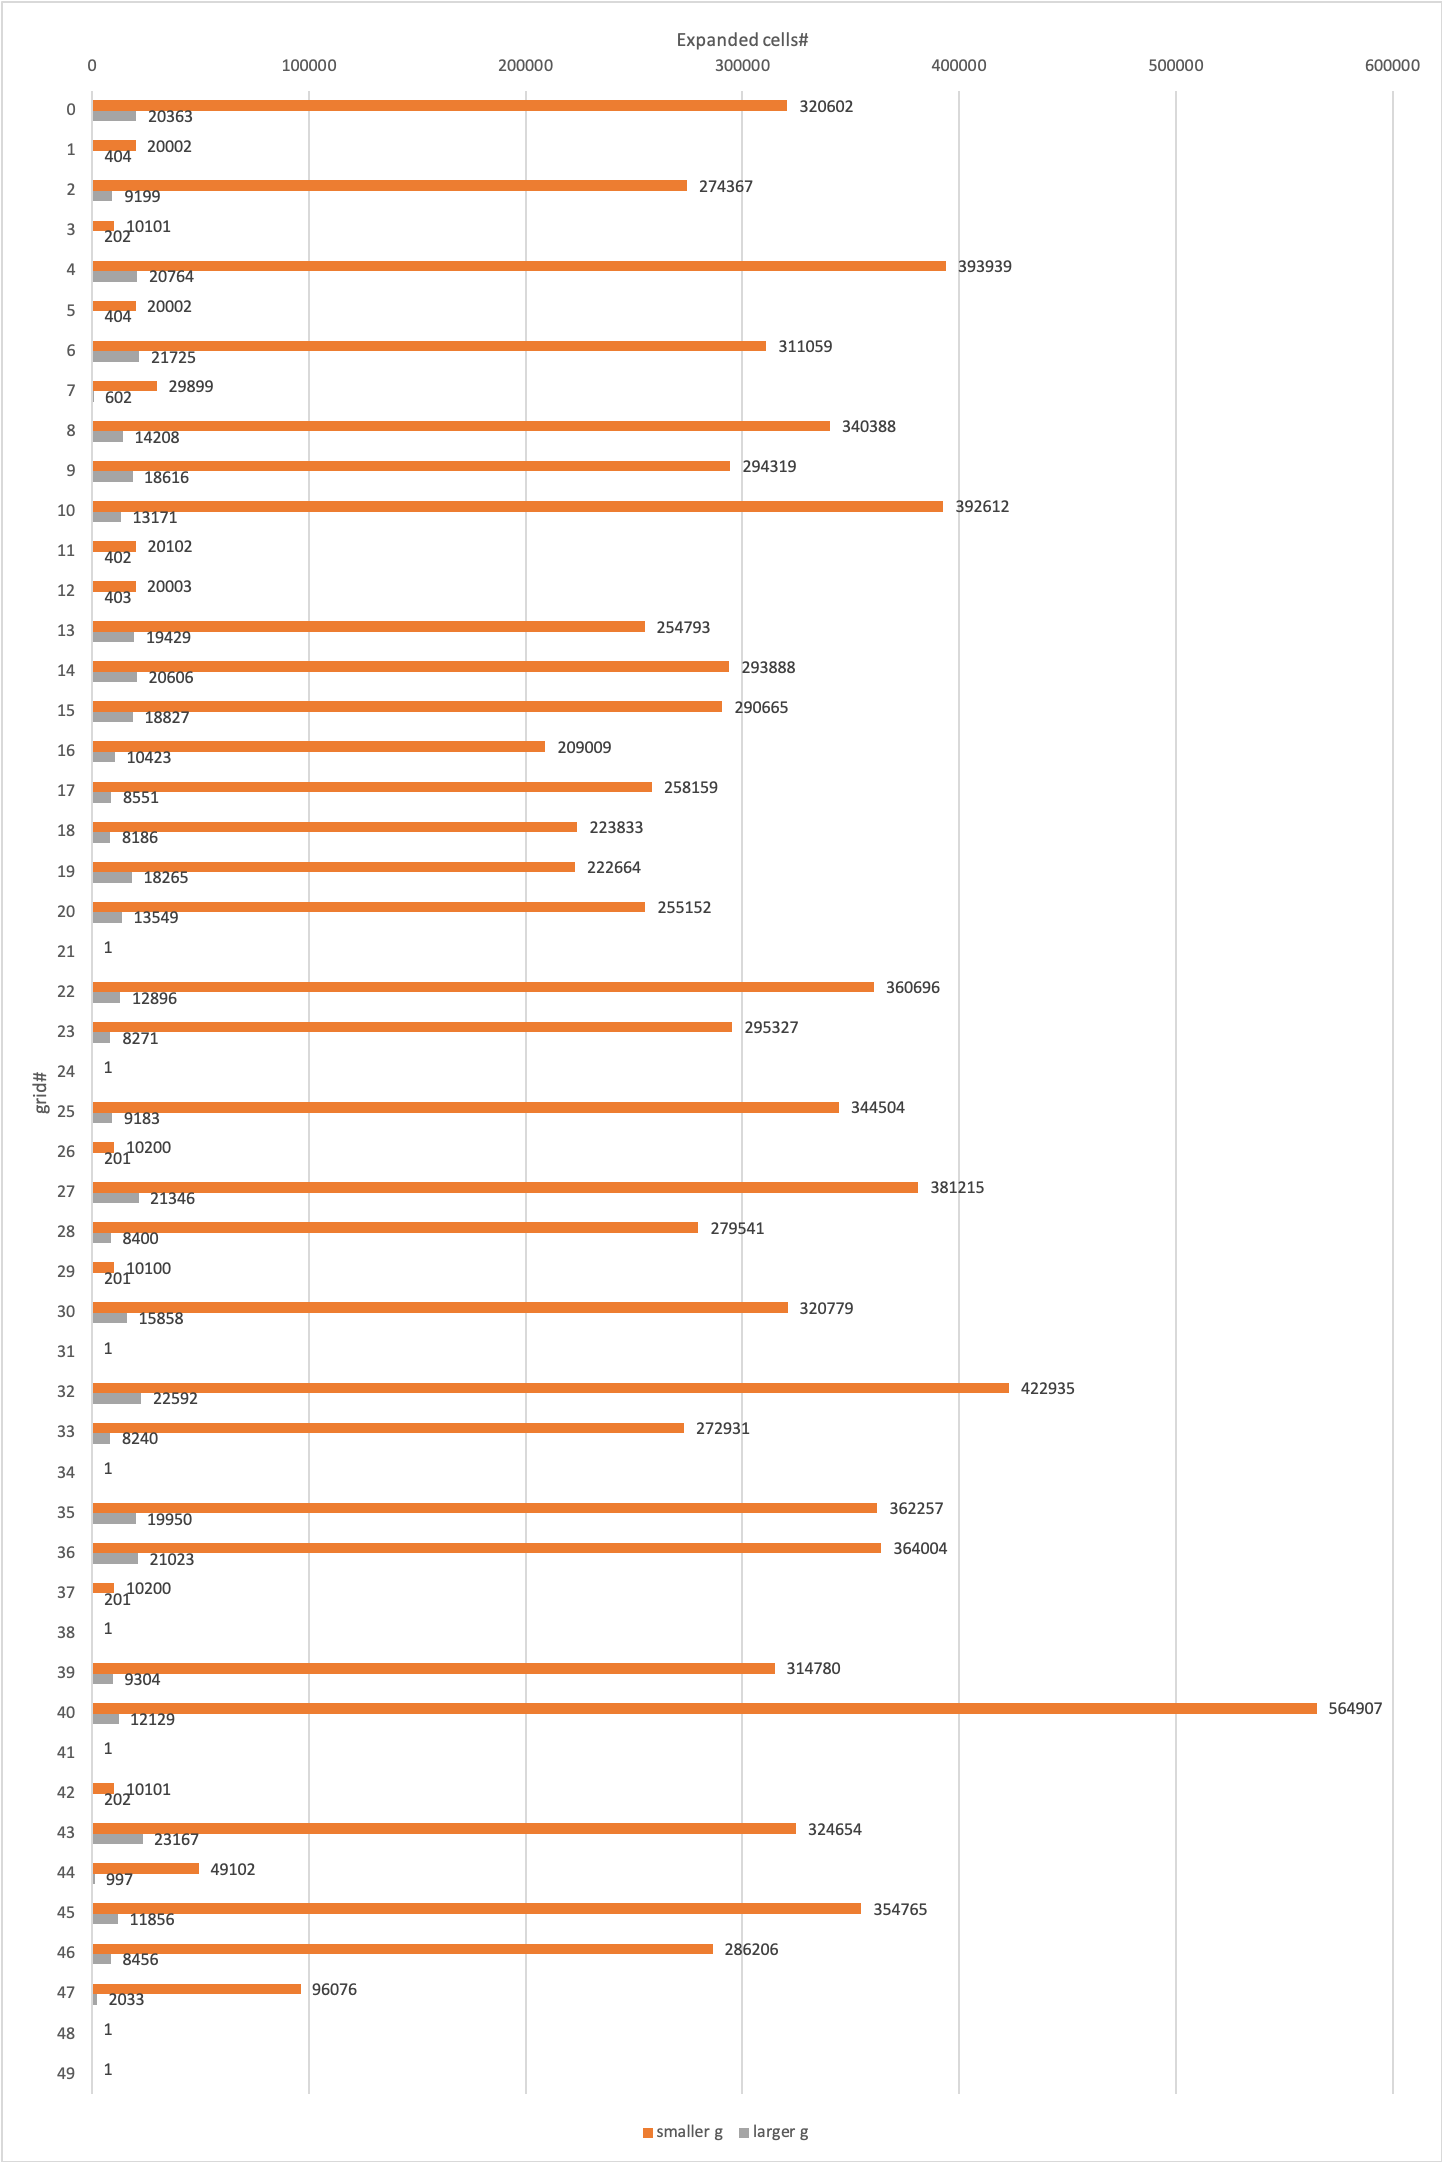
\includegraphics[scale=0.47]{part2}
\caption{Breaking Ties in Favour of Smaller g-values vs Larger g-values}
\label{part2}
\end{figure}

\paragraph*{}
From figure \ref{part2} we can observe when we break ties in favour of cells with smaller g-values, the number of expanded cells is way larger than when we break ties in favour of larger g-values.

\paragraph*{}
The reason is that favouring smaller g-values means favouring cells closer to the start cell, but will lager h-values compare to other cells with the same f-values, which means they are farther away from the goal cell. Hence, bad paths are expanded first, leads to more cells being expanded, and results in greater runtime than favouring larger g-values.

\newpage 
\section*{Part 3}

\begin{figure}
\centering
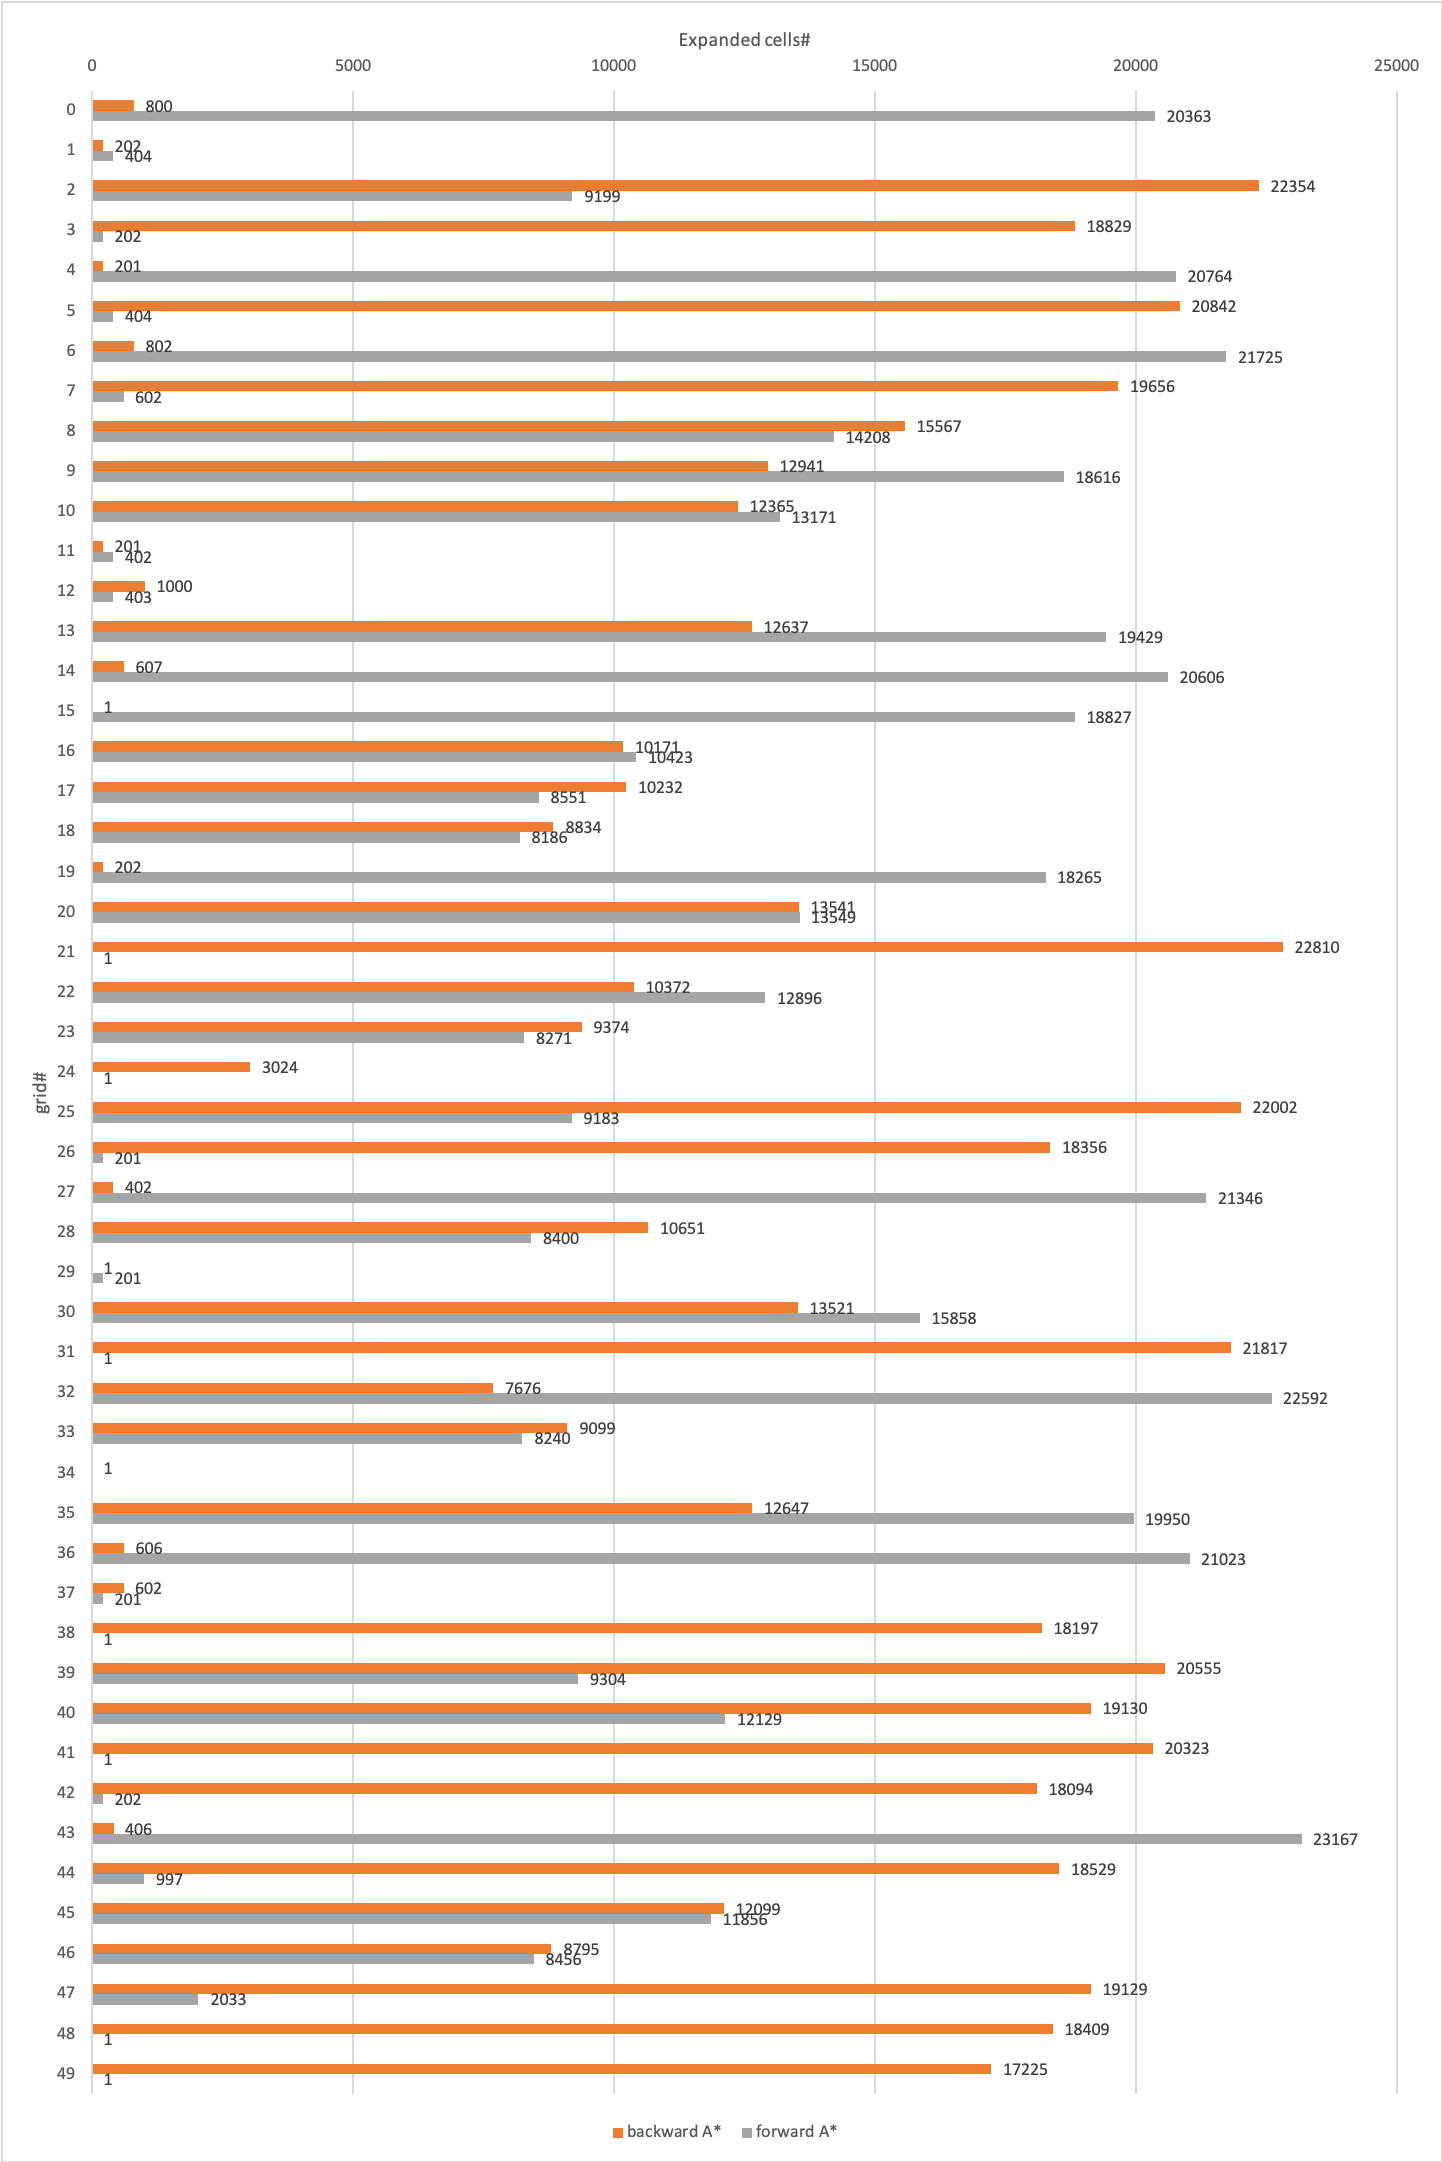
\includegraphics[scale=0.47]{part3.1}
\caption{Repeated Forward vs Backward A* With Ties Breaking}
\label{part3.1}
\end{figure}

\begin{figure}
\centering
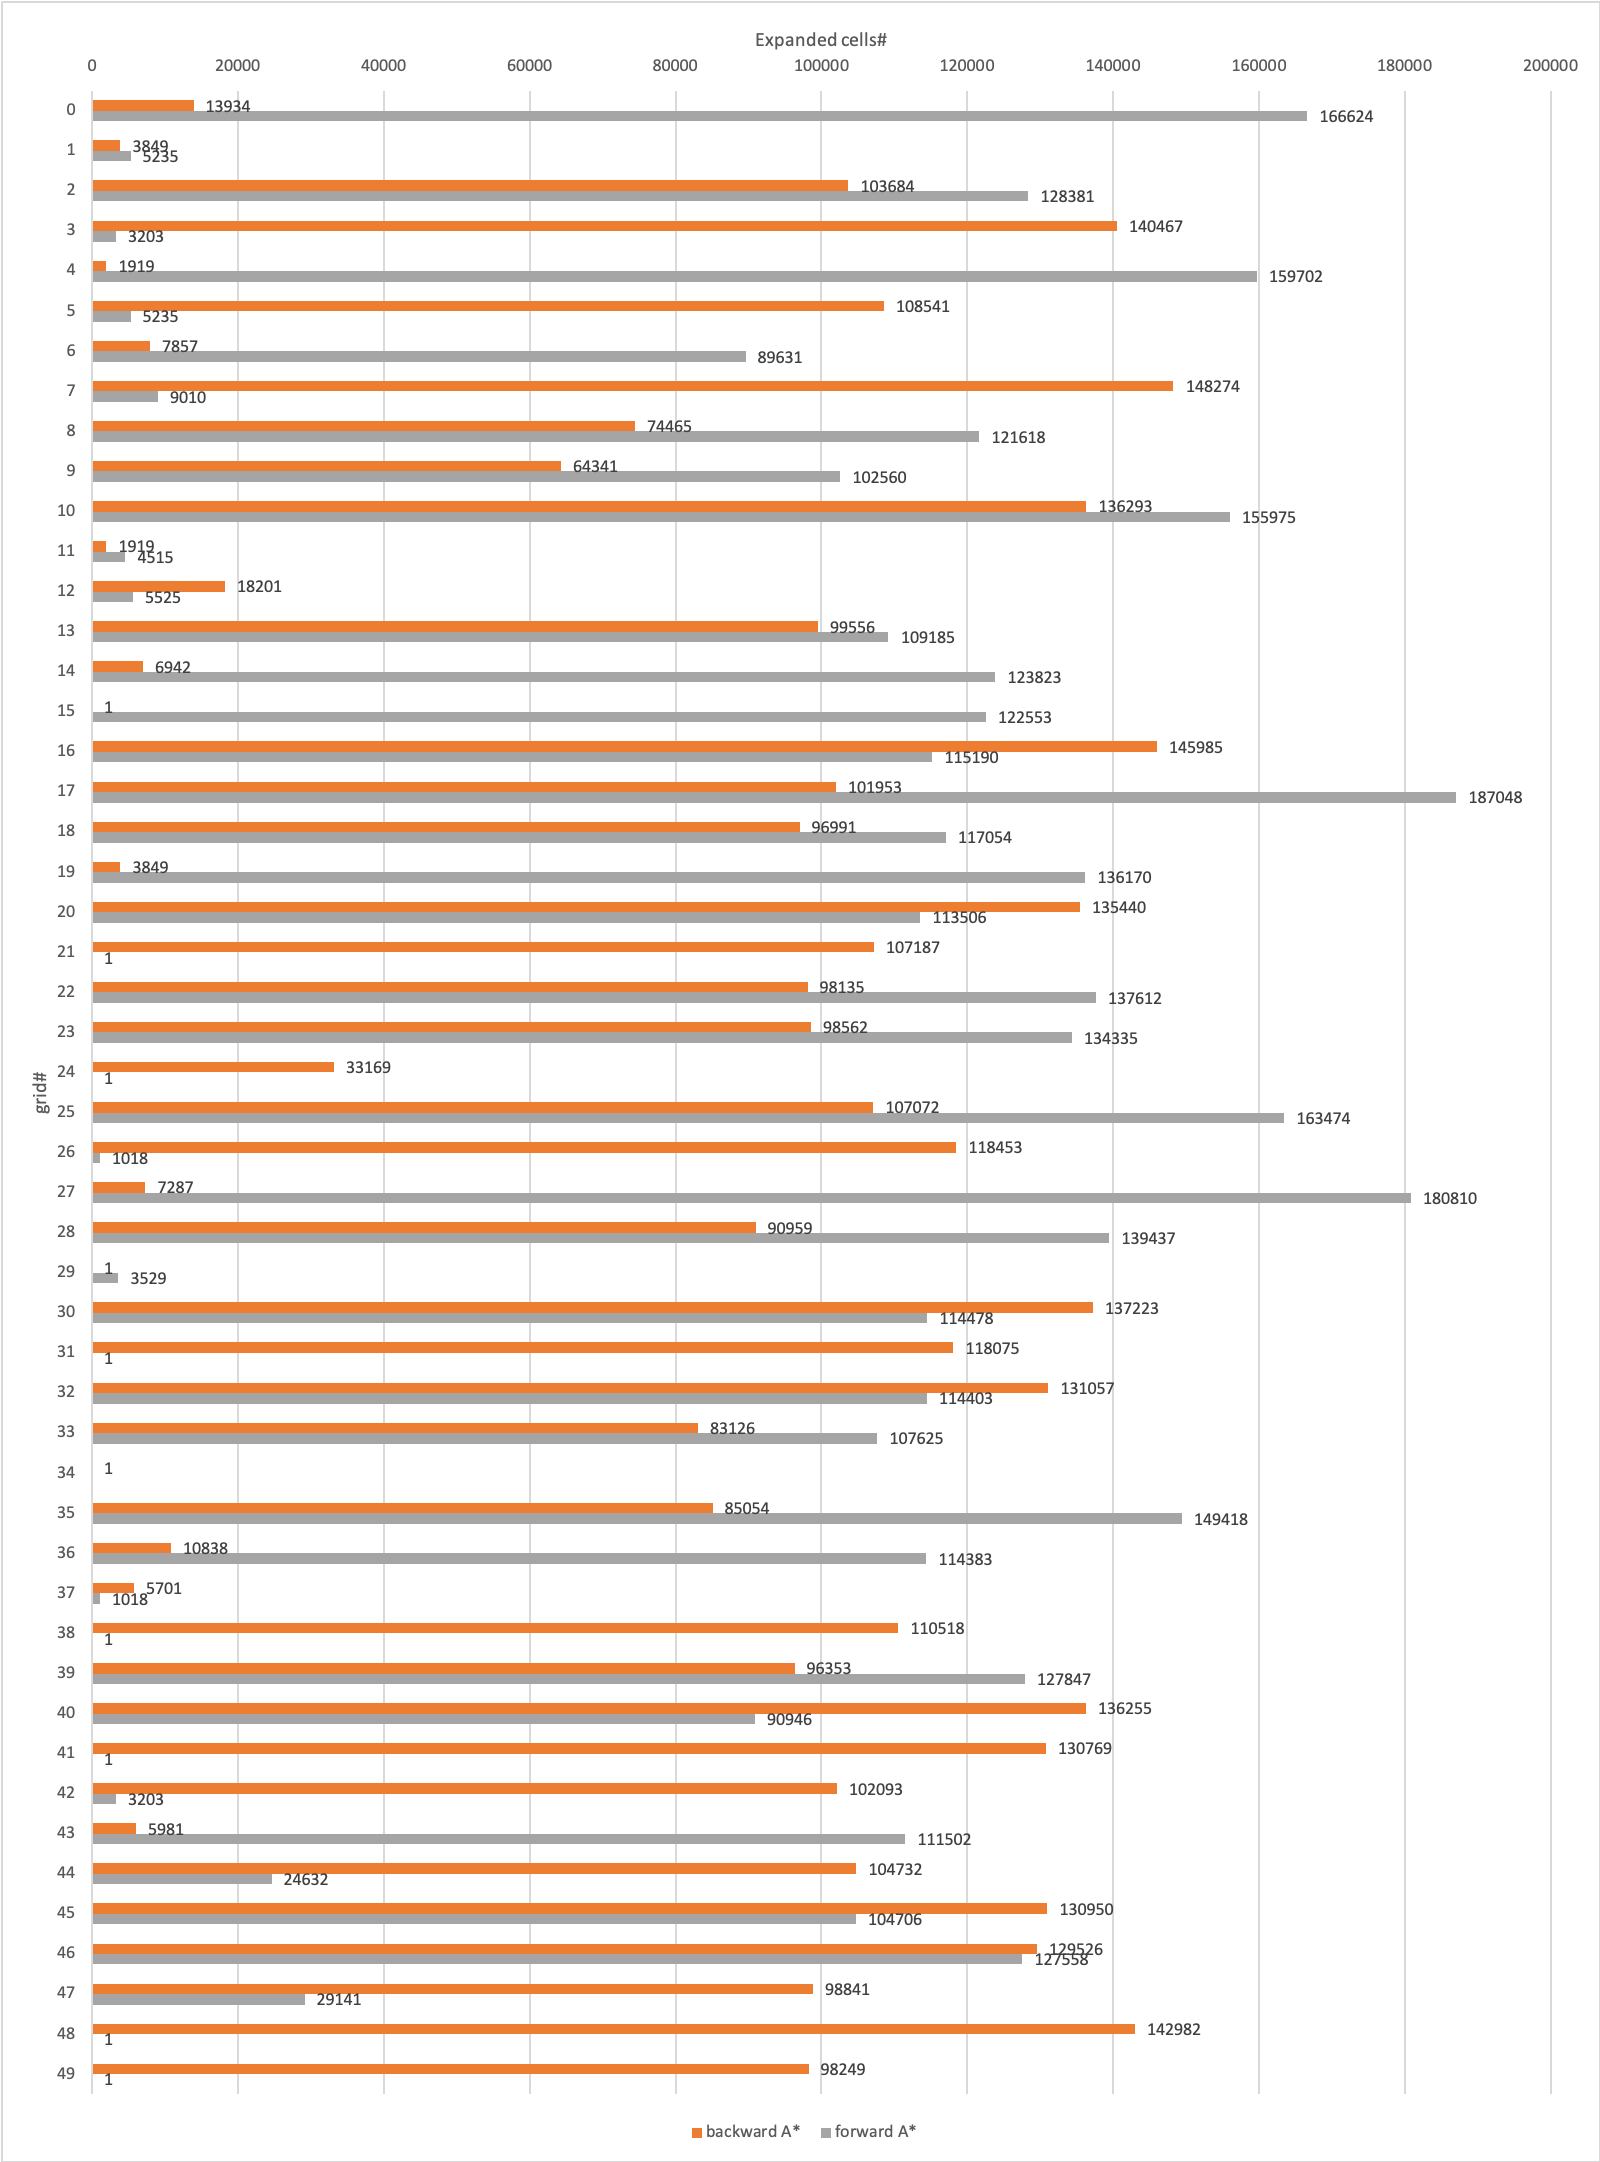
\includegraphics[scale=0.47]{part3.2}
\caption{Repeated Forward vs Backward A* With Ties Remained}
\label{part3.2}
\end{figure}

\begin{figure}
\centering
\subfigure[grid 15]{
\label{grid15}
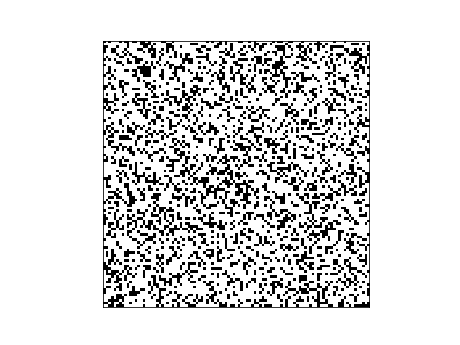
\includegraphics[scale=0.46]{maze15}}
\subfigure[grid 34]{
\label{grid34}
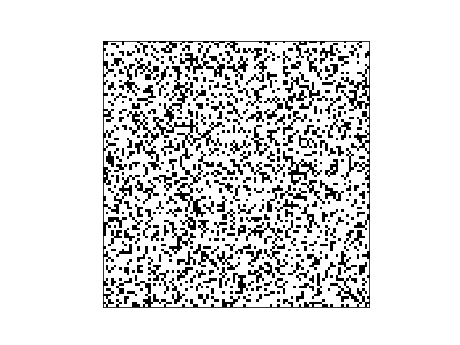
\includegraphics[scale=0.46]{maze34}}
\subfigure[grid 49]{
\label{grid49}
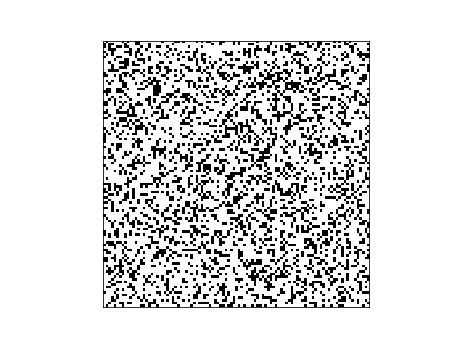
\includegraphics[scale=0.46]{maze49}}
\caption{Randomly Generated Grids}
\label{grids}
\end{figure}

\paragraph*{}
From figure \ref{part3.1} we can observe that repeated backward A* can be faster or slower than repeated forward A* depends on which grid they are searching on. Any by comparing figure \ref{part3.1} and figure \ref{part3.2} we can know that A* with ties breaking is faster than A* without ties breaking. Below we will pick grid 15, 34 and 49 to analyse in detail to compare repeated forward and backward A*.

\paragraph*{}
In grid 34, cells around both the start and the end are blocked, so both forward and backward A* found it is impossible to reach end from start.
In grid 15, cells around the end are blocked but around the start are opened, so it took more time for forward A* to discover it is impossible to reach the end.
In grid 49, cells around the start are blocked but around the end are opened, so it took more time for backward A* to discover it is impossible to reach the start.

\paragraph*{}
In conclusion, whether backward A* will be faster than forward A* depends on whether the possible path around the end is more limited than the start, such that backward A* will have less cells to expanded. But breaking ties can significantly improve the runtime of both forward and backward A*.

\newpage
\section*{Part 4}

\subsection*{a)}
\paragraph*{}
If the heuristic is calculated using Manhattan distances:
$$h(s) = |x_s - x_{s_{goal}}| + |y_s-y_{s_{goal}}|$$
$$h(s_{goal}) = |x_{s_{goal}} - x_{s_{goal}}| + |y_{s_{goal}}-y_{s_{goal}}| = 0$$

\paragraph*{}
Since the agent can move only in the four main compass directions, to move from cell $s_1$ to cell $s_2$, the number of actions in vertical directions $y \ge |y_{s_1} - y_{s_2}|$. Similarly, the number of actions in horizontal directions $x \ge |x_{s_1} - x_{s_2}|$. \\
The total cost of moving from cell $s_1$ to cell $s_2$
\begin{equation}\label{eq:cost}
c(s_1, a, s_2) = x + y \ge |x_{s_1} - x_{s_2}| + |y_{s_1} - y_{s_2}|
\end{equation}

\begin{equation*}
\begin{split}
|x_{s_1} - x_{s_2}| + |y_{s_1} - y_{s_2}| &= |(x_{s_1} - x_{s_{goal}}) - (x_{s_2} - x_{s_{goal}})| + |(y_{s_1} - x_{s_{goal}}) - (y_{s_2} - x_{s_{goal}})|\\
&\ge |(x_{s_1} - x_{s_{goal}})| - |(x_{s_2} - x_{s_{goal}})| + |(y_{s_1} - x_{s_{goal}})| - |(y_{s_2} - x_{s_{goal}})|\\
&= |(x_{s_1} - x_{s_{goal}})| + |(y_{s_1} - x_{s_{goal}})| - |(x_{s_2} - x_{s_{goal}})| - |(y_{s_2} - x_{s_{goal}})|\\
&= h(s_1) - h(s_2)
\end{split}
\end{equation*}
$$c(s_1, a, s_2) \ge h(s_1) - h(s_2)\Longrightarrow h(s_1) \le c(s_1, a, s_2) + h(s_2)$$

\paragraph*{}
Hence, The Manhattan distances are consistent.

\subsection*{b)}

\paragraph*{}
Let $g(s)$ be the Manhattan distance from the start state to state $s$.\\
We can rewrite \eqref{eq:cost} as the following equation:
$$c(s_1, a, s_2) \ge g(s_2) - g(s_1)$$
The new h-values are calculated using the following equation:
\begin{equation*}
	\begin{split}
		h_{new}(s_1) &= g(s_{goal}) - g(s_1) \\
		&= (g(s_{goal}) - g(s_2)) - (g(s_1) - g(s_2)) \\
		&= h_{new}(s_2) + (g(s_2) - g(s_1)) \le h_{new}(s_2) + c(s_1, a, s_2)
	\end{split}
\end{equation*}
$$h_{new}(s_1) \le h_{new}(s_2) + c(s_1, a, s_2)$$
And the above inequality is still valid even if $c(s_1, a, s_2)$ can increase. For $g_{goal}$:
$$h_{new}(g_{goal}) = g(s_{goal}) - g(s_{goal}) = 0$$
Hence, $h_{new}(s)$ is consistent even if action costs can increase.

\section*{Part 5}

After completing Adaptive A* on 50 maps, we discovered that the average nodes expanded were 3423.6, the average amount of time spent on execution was 0.001202671979999934 sec, and the average amount of memory was 3.9162400000000005e-09 mb.\\
On the other hand, after completing Forward A* on 50 maps, we discovered that the average nodes expanded were 3637.6, the average amount of time spent on execution was 1.6033800000059274e-06 sec, and the average amount of memory was 1.784e-11 mb.\\ 
\bigskip{}
As we can see, adaptive is on average less memory intensive and also faster then repeated forward A*. This is because Adaptive A* updates the h values of expanded cells to a higher value that is consistent. This new h value is more accurate after each iteration of A*. After these values are added to the open list again, Adaptive A* to make better choices in movement and planning. Ultimately, the number of cells expanded by Adaptive A* will be less than ordinary A*. This ultimately makes it a generally faster program.

\section*{Part 6}

\bigskip{\bf{Ways of making the program more memory efficient:}}
\bigskip{}

1.) Reduce amount of information stored state class:\\
In our program, we use the a state class has many instance variables attached to it. Each instance of the state class produced must inherit and store data in each of these variables. A way to potentially accomplish this would be either eliminate or reduce variable size. Since, search instance variable in the state class only needs to be checked to make sure that a state has been visited already, these could potentially be converted to booleans instead of integers.\\
\bigskip{}
2.) Using generator functions can reduce memory consumption:\\
Generator functions do not sore results in memory, they return values on the fly. By using generator functions such as when computing the children of a state, we can avoid returning a list which occupies memory. \\

\bigskip{}
3.) Removing redundant arrays:\\
There are definitely redundant arrays in the code that could either be combined with other arrays or removed entirely. For instance in adaptive a* there are 2 closed lists, one containing states and the other containing tuples (position). We could remove the tuple list as it is not as important to program function. This would free up memory. \\
\bigskip{\bf{Calculate the amount of memory that they need to operate on grids of size 1001*1001}}
\bigskip{}
- Each state has a list of children that contains at most 4 size 2 tuples. The maximum memory size is 96 bytes.\\

- Each state has two pointers which are 4 bytes each \\ 

 - Each state has a single tuple for pos which is 24 bytes\\
 
 - Each state has 4 integers for f,h,g,search = 24 bytes\\
 
 - Each state has another boolean in\_open = 1 byte \\
 
 - 96 + 8 + 64 + 24 + 1 = 153 bytes
 1001 * 1001 * 193 = 153306153 bytes
 
\bigskip{\bf{Calculate the largest grid that they can operate on within a memory limit of 4 MBytes}}\\
- since each cell is 193 bytes \\
$\frac{4 * 1001}{193}$ = $26$

\end{document}
